\section{An Example}

In this section, the proposed algorithm will be applied to the example graph \(G\) (\(n=8\) and \(m=12\)) shown in
Figure \ref{fig:example} in order to determine its chromatic number.  The steps of the algorithm are then traversed
in reverse order to determine a chromatic coloring.

\begin{figure}[h]
  \label{fig:example}
  \begin{center}
    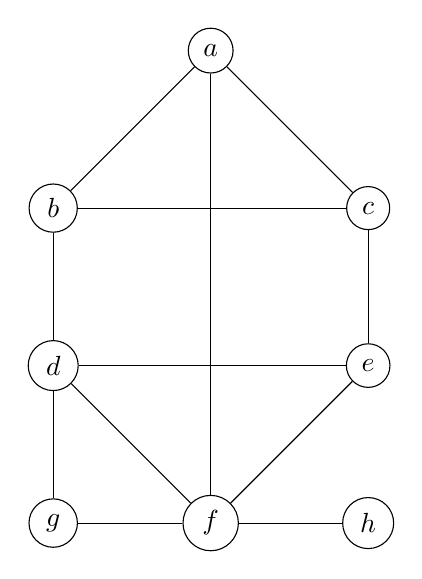
\begin{tikzpicture}
      \node (a) [draw,circle] at (2,6) {\(a\)};
      \node (b) [draw,circle] at (0,4) {\(b\)};
      \node (c) [draw,circle] at (4,4) {\(c\)};
      \node (d) [draw,circle] at (0,2) {\(d\)};
      \node (e) [draw,circle] at (4,2) {\(e\)};
      \node (f) [draw,circle] at (2,0) {\(f\)};
      \node (g) [draw,circle] at (0,0) {\(g\)};
      \node (h) [draw,circle] at (4,0) {\(h\)};
      \draw (a) to (b);
      \draw (a) to (c);
      \draw (a) to (f);
      \draw (b) to (c);
      \draw (b) to (d);
      \draw (c) to (e);
      \draw (d) to (e);
      \draw (d) to (f);
      \draw (d) to (g);
      \draw (e) to (f);
      \draw (f) to (g);
      \draw (f) to (h);
    \end{tikzpicture}
  \end{center}
  \caption{Example Graph}
\end{figure}

The algorithm steps are as follows.  Outer loop steps are marked by ``O\#'' and called subroutine steps are marked by
``I\#.''.  Recursive subroutine calls add a call level: ``I\#--\#.''

\begin{enumerate}
\item (O\ref{step:null}) Since \(n=8>0\), \(G\) is not the null graph, so continue.

\item (O\ref{step:one}) Since \(n=8>1\), \(G\) is not an empty graph, so continue.

\item (O\ref{step:init}) Initialize \(k\) to 2.

\item (O\ref{step:inner}) Call the subroutine with \(G\) and \(k=2\).

\item (I\ref{step:check}) \(n=8>k=2\), so continue.

\item (I\ref{step:dencalc}) Calculate the maximum edge threshold for \(n=8\) and \(k=2\):
  \[a=\frac{n^2(k-1)}{2k}=\frac{8^2(2-1)}{2\cdot2}=\frac{64}{4}=16\]

\item (I\ref{step:density}) Since \(m=12\ngtr16=a\), continue.

\item (I\ref{step:smallcalc}) Note that \(\deg{h}=1<2\), so let \(X=\set{h}\).

\item (I\ref{step:small}) Since \(X\ne\emptyset\), replace \(G\) with \(G-X\).  The result is shown in Figure
  \ref{fig:removeh}.  Now \(n=7\) and \(m=11\).

  \begin{figure}[h]
    \label{fig:removeh}
    \begin{center}
      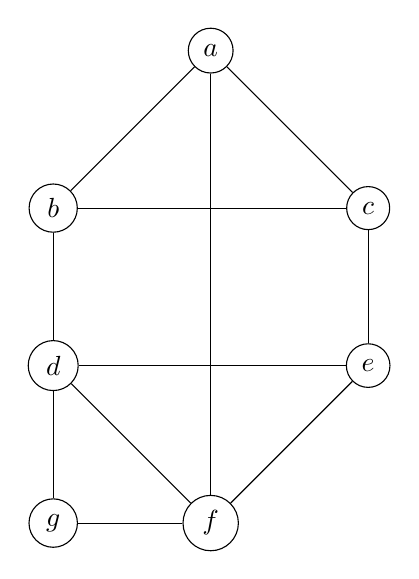
\begin{tikzpicture}
        \node (a) [draw,circle] at (2,6) {\(a\)};
        \node (b) [draw,circle] at (0,4) {\(b\)};
        \node (c) [draw,circle] at (4,4) {\(c\)};
        \node (d) [draw,circle] at (0,2) {\(d\)};
        \node (e) [draw,circle] at (4,2) {\(e\)};
        \node (f) [draw,circle] at (2,0) {\(f\)};
        \node (g) [draw,circle] at (0,0) {\(g\)};
        \draw (a) to (b);
        \draw (a) to (c);
        \draw (a) to (f);
        \draw (b) to (c);
        \draw (b) to (d);
        \draw (c) to (e);
        \draw (d) to (e);
        \draw (d) to (f);
        \draw (d) to (g);
        \draw (e) to (f);
        \draw (f) to (g);
      \end{tikzpicture}
    \end{center}
    \caption{\(G-\set{h}\)}
  \end{figure}

\item (I\ref{step:check}) \(n=7>k=2\), so continue.

\item (I\ref{step:dencalc}) Calculate the maximum edge threshold for \(n=7\) and \(k=2\):
  \[a=\frac{n^2(k-1)}{2k}=\frac{7^2(2-1)}{2\cdot2}=\frac{49}{4}=12.25\]

\item (I\ref{step:density}) Since \(m=12\ngtr12.25=a\), continue.

\item (I\ref{step:smallcalc}) Since \(\d(G)=2\ge2=k\), set \(X=\emptyset\).

\item (I\ref{step:small}) Since \(X=\emptyset\), continue.

\item (I\ref{step:neighbor}) Note that \(N(g)=\set{d,f}\) and \(N(e)=\set{c,d,f}\).  Since \(N(g)\subseteq N(e)\),
  replace \(G\) with \(G-g\).  The result is shown in Figure \ref{fig:removeg}.  Now \(n=6\) and \(m=9\).

  \begin{figure}[h]
    \label{fig:removeg}
    \begin{center}
      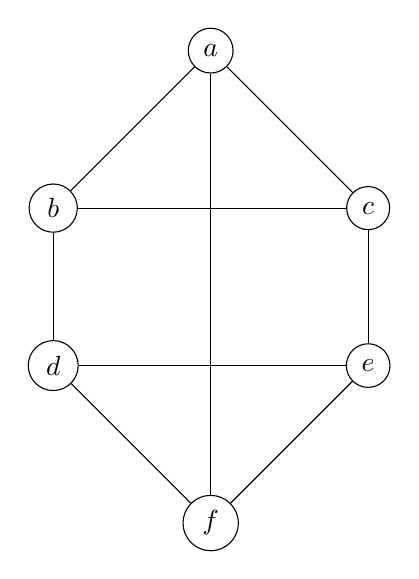
\begin{tikzpicture}
        \node (a) [draw,circle] at (2,6) {\(a\)};
        \node (b) [draw,circle] at (0,4) {\(b\)};
        \node (c) [draw,circle] at (4,4) {\(c\)};
        \node (d) [draw,circle] at (0,2) {\(d\)};
        \node (e) [draw,circle] at (4,2) {\(e\)};
        \node (f) [draw,circle] at (2,0) {\(f\)};
        \draw (a) to (b);
        \draw (a) to (c);
        \draw (a) to (f);
        \draw (b) to (c);
        \draw (b) to (d);
        \draw (c) to (e);
        \draw (d) to (e);
        \draw (d) to (f);
        \draw (e) to (f);
      \end{tikzpicture}
    \end{center}
    \caption{\(G-g\)}
  \end{figure}

\item (I\ref{step:check}) \(n=6>k=2\), so continue.

\item (I\ref{step:dencalc}) Calculate the maximum edge threshold for \(n=6\) and \(k=2\):
  \[a=\frac{n^2(k-1)}{2k}=\frac{6^2(2-1)}{2\cdot2}=\frac{36}{4}=9\]

\item (I\ref{step:density}) Since \(m=9\ngtr9=a\), continue.

\item (I\ref{step:smallcalc}) Since \(\d(G)=2\ge2=k\), set \(X=\emptyset\).

\item (I\ref{step:small}) Since \(X=\emptyset\), continue.

\item (I\ref{step:neighbor}) Since there is no \(N(u)\subseteq N(v)\), continue.

\item (I\ref{step:select}) Note that due to the symmetry of \(G\) every two vertices share exactly two neighbors:
  \[b=\min_{u,v\in V(G)}\abs{N(u)\cap N(v)]}=2\]

\item (I\ref{step:neighcalc}) Calculate the upper bound for minimum number of common neighbors for \(n=6\) and
  \(k=2\):
  \[c=n-2-\frac{n-2}{k-1}=6-2-\frac{6-2}{2-1}=4-4=0\]

\item (I\ref{step:common}) Since \(b=2>0=c\), conclude that \(G\) is not \colorable{2}.  Return false and the current
  state of \(G\) to the outer loop.

\item (O\ref{step:call}) Since the called subroutine returned false, \(G\) is not \colorable{2}, so continue.

\item (O\ref{step:newg}) Replace \(G\) with the graph returned by the previous call (Figure \ref{fig:removeg}).

\item (O\ref{step:incr}) Increment \(k\) to 3.

\item (O\ref{step:inner}) Call the subroutine with the new \(G\) and \(k=3\).
  
\item (I\ref{step:check}) \(n=6>k=3\), so continue.

\item (I\ref{step:dencalc}) Calculate the maximum edge threshold for \(n=6\) and \(k=3\):
  \[a=\frac{n^2(k-1)}{2k}=\frac{6^2(3-1)}{2\cdot3}=\frac{72}{6}=12\]

\item (I\ref{step:density}) Since \(m=9\ngtr11=a\), continue.

\item (I\ref{step:smallcalc}) Since \(\d(G)=3\ge3=k\), set \(X=\emptyset\).

\item (I\ref{step:small}) Since \(X=\emptyset\), continue.

\item (I\ref{step:select}) Note that due to the symmetry of \(G\) every two nodes share exactly two neighbors:
  \[b=\min_{u,v\in V(G)}\abs{N(u)\cap N(v)]}=2\]

\item (I\ref{step:neighcalc}) Calculate the upper bound for minimum number of common neighbors for \(n=6\) and
  \(k=3\):
  \[c=n-2-\frac{n-2}{k-1}=6-2-\frac{6-2}{3-1}=4-2=2\]

\item (I\ref{step:common}) Since \(b=2\ngtr2=c\), continue.

\item (I\ref{step:select2}) Since every two vertices share exactly two neighbors, select any two non-adjacent
  vertices: \(a\) and \(c\).

\item (I\ref{step:call1}) Recursively call the subroutine with \(G\cdot ac\) and \(k=3\).  The result is shown in
  Figure \ref{fig:conac}.

  \begin{figure}[h]
    \label{fig:conac}
    \begin{center}
      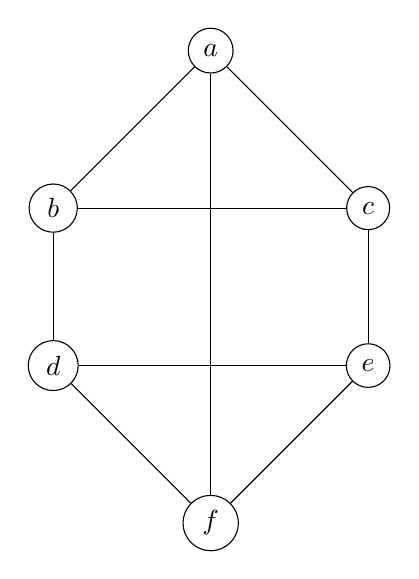
\begin{tikzpicture}
        \node (a) [draw,circle] at (2,6) {\(a\)};
        \node (b) [draw,circle] at (0,4) {\(b\)};
        \node (c) [draw,circle] at (4,4) {\(c\)};
        \node (d) [draw,circle] at (0,2) {\(d\)};
        \node (e) [draw,circle] at (4,2) {\(e\)};
        \node (f) [draw,circle] at (2,0) {\(f\)};
        \draw (a) to (b);
        \draw (a) to (c);
        \draw (a) to (f);
        \draw (b) to (c);
        \draw (b) to (d);
        \draw (c) to (e);
        \draw (d) to (e);
        \draw (d) to (f);
        \draw (e) to (f);
      \end{tikzpicture}
    \end{center}
    \caption{\(G-g\)}
  \end{figure}
\end{enumerate}
